\def\year{2018}\relax
%File: formatting-instruction.tex
\documentclass[letterpaper]{article}
\usepackage{aaai17}
\usepackage{times}
\usepackage{multirow}
\usepackage{helvet}
\usepackage{courier}
\usepackage{amsmath}
\usepackage{graphicx}
\usepackage{amssymb}
\usepackage{algorithm}
\usepackage[noend]{algpseudocode}
\usepackage{url}
\usepackage{subcaption}
\newcommand{\smallurl}[1]{\scriptsize{\url{#1}}}
\usepackage{verbatim}
\usepackage{multirow}
\usepackage{tabularx}
\usepackage[normalem]{ulem}
\usepackage{float}
\DeclareMathAlphabet\mathbfcal{OMS}{cmsy}{b}{n}
% Use the postscript times font!
\usepackage{times}
\newenvironment{smallenum}{\setlength{\topsep}{0.0 truein}\begin{enumerate} 
   \setlength{\leftmargin}{.25 truein}
   \setlength{\parsep}{0.0 truein}
   \setlength{\parskip}{0.0 truein}
   \setlength{\itemsep}{0.0 truein}}{\end{enumerate}}
\newenvironment{smalldesc}{\setlength{\topsep}{0.0 truein}\begin{description} 
   \setlength{\leftmargin}{.25 truein}
   \setlength{\parsep}{0.0 truein}
   \setlength{\parskip}{0.0 truein}
   \setlength{\itemsep}{0.0 truein}}{\end{description}}
\usepackage[dvipsnames]{xcolor}
%known valid colors include: red, blu, ForestGreen, cyan, DarkOrchid
\newcommand{\fromsach}[1]{\frombody{blue}{Sachini}{#1}}
\newcommand{\frommak}[1]{\frombody{ForestGreen}{Mak}{#1}}
\newcommand{\fromnotes}[1]{\frombody{DarkOrchid}{Notes}{#1}}
%Use the empty command below to hide all comments
\newcommand{\frombody}[3]{\noindent\textcolor{#1}{{$\bf [\![\!\![$}\underline{\scshape{#2}} {\scshape says:} \textsl{#3}{$\bf ]\!\!]\!]$}}}
%uncomment the following line to hide \fromXXX comments prior to publishing
%\renewcommand{\frombody}[3]{}

%mak: list with no symbol
\newenvironment{simplelist}{
 \begin{list}{}
  {\setlength{\itemsep}{1pt}
   \setlength{\parsep}{1pt}
   \setlength{\topsep}{2pt}
   \setlength{\partopsep}{1pt}
   \setlength{\leftmargin}{3em}
   \setlength{\labelwidth}{3em}
   \setlength{\labelsep}{0.6em}}}
  {\end{list}}
%mak: list with a dash
\newenvironment{dashlist}{
 \begin{list}{-}
  {\setlength{\itemsep}{0pt}
   \setlength{\parsep}{0pt}
   \setlength{\topsep}{0pt}
   \setlength{\partopsep}{1pt}
   \setlength{\leftmargin}{1.5em}
   \setlength{\labelwidth}{2em}
   \setlength{\labelsep}{0.6em}}}
  {\end{list}}


\usepackage{amsthm}
\theoremstyle{plain}
\newtheorem{definition}{Definition}


\frenchspacing
\setlength{\pdfpagewidth}{8.5in}
\setlength{\pdfpageheight}{11in}
% exclude the submission because meta data would violate blind review
%\pdfinfo{
%/Title (Domain-independent Plan Intervention)
%/Author (Sachini Weerawardhana, Darrell Whitley, Mark Roberts)}
\setcounter{secnumdepth}{2}  
\begin{document}
\title{Domain-independent Plan Intervention}
%\author{ Paper \#204}
%\author{
% \large{\bf{
%Sachini Weerawardhana\and Darrell Whitley$^1$ Mark Roberts$^2$}} \\
%\small{$^1$Computer Science Department, Colorado State University, Fort Collins, CO, USA $\mid$ \{sachini, whitley\}@cs.colostate.edu} \\
%\small{$^2$The U.S. Naval Research Laboratory, Code 5514; Washington, DC, USA $\mid$ mark.roberts@nrl.navy.mil}\\ 
% }
%put questions under this command. fix before submission
%arg1 = owner of comment arg2 = TODO/comment
\newcommand{\debug}[2]{[\textbf{DEBUG #1}: \textcolor{WildStrawberry}{\textit{#2}}]}
\nocopyright
\maketitle
\begin{abstract}
%broad statement of how this work is applicable
Intervening is common in online assistive agents (e.g., route planning, tutoring) and safety-critical decision making (e.g., cybersecurity, medical diagnosis), where an observer determines how to guide a user toward a desirable outcome while avoiding undesirable outcomes.
%what's the gap this work addresses
In the planning domain, intervention requires a slightly different perspective from the standard formulation of plan recognition because the observer needs to account for the goals of the user as well as undesirable outcomes (sometimes inserted by an competing agent) about which the user may be unaware.
%how does this work address this gap? what is the technical contribution?
We formalize the plan intervention problem and introduce the Intervention Graph, which characterizes the observer's decision space.
We propose domain-independent features extracted or sampled from the Intervention Graph to measure the criticality of an action leading to undesirable outcomes.
We apply these features to four learning algorithms that learn whether to intervene in online scenarios with varying undesirable outcomes.
%how do you evaluate the approach?
In an evaluation of several benchmark problems, including one we introduce called Rush Hour,
%what are the findings?
the learned models outperform, sometimes substantially, three recent plan recognition approaches in most problems, although the performance varies by the application.
%summing up: what are the implications? who cares?
To our knowledge, this is the first work to incorporate recent plan recognition techniques into plan intervention.
Our work lays a foundation for further applications of assistive and decision support agents.
\end{abstract}

%=========================================================================
%=========================================================================
%=== intro
%=========================================================================
%=========================================================================
\section{Introduction}\label{sec:intro}
Even the best plan can be misguided.
Dangers might arise from a user failing to follow the plan correctly or as a result of a nefarious agent.
A safe plan might still be misguided when a better, but unknown, alternative exists.
Consider route planning where a driver was unaware of upcoming road damage or a traffic jam.  
Or consider cybersecurity where a user was unaware of an unsafe hyperlink.
In both, plans achieving the desirable goal (e.g., arriving at the destination, checking email) might have similar prefixes to those that result in undesirable outcomes (e.g., hitting a pothole, clicking on a phishing link); only the plan suffix differs.
State-of-the-art goal recognition techniques only provide a part of the solution for selecting interventions.
%% Intervention can thus be used to avoid negative outcomes or provide hints if a user is stuck.
%need to lead into intervention for the rush hour domain
%% We define ``safety'' as a charactisic of a plan for a human ``user.''
%% define criticality
%% deemphasize the attacker's role (only one problem fits, after all)

In this work, we create a domain-independent formulation of learning \emph{whether} to intervene.
At a minimum, intervention problems require a user and some intervening observer.
In adversarial settings, intervention also requires an competing agent.
%In either case, the ideal observer would intervene early.  

Since plans to desirable and undesirable outcomes could overlap, there is a tradeoff between mitigating the undesirable outcome while allowing the user some freedom.  
Reducing intrusion and allowing more freedom are reasonable for assistive agents where a misstep is correctable and its cost is comparatively low (e.g., a GPS route planner, an online tutor) but could be disastrous when an undesirable outcome cannot be undone and its cost is high (e.g., medical diagnosis, cybersecurity).  
We focus on one extremum of this tradeoff---i.e., minimizing user annoyance at the cost of sometimes missing critical actions---and examine how to determine whether to intervene with the assumption that late intervention is better than none at all.
The contributions of this paper include:
\begin{itemize}
\item extending an existing plan recogintiion model to support the intervention problem;
\item formalizing the online intervention problem as determining when the criticality--i.e., the opportunity or urgency of possible damage--of a state warrants interruption; 
\item modeling the observer's decision space as an \emph{Intervention Graph}, which can be constructed explicitly or sampled with the TopK planner (Riabov et al., \citeyear{riabov2014});
\item defining domain-\emph{independent} features to assess the criticality of a state using the Intervention Graph;
\item extending existing goal/plan recognition benchmarks \cite{ramirez2009plan,ramirez2010probabilistic} to incorporate intervention and introducing a new plan intervention benchmark domain called Rush Hour\footnote{We will release these benchmarks and code upon publication}, 
\item adapting four algorithms that learn whether to intervene, 
\item comparing these learning algorithms against three state-of-the-art goal recognition techniques, and
\item demonstrating that all learning methods dominate when using the intervention graph features and perform better or comparably using sampled features.
\end{itemize}
Our results suggest a tradeoff between the features and algorithms used for intervention, that this tradeoff is benchmark specific, and provide a foundation from which future work on online plan intervention can build.


\section{Background: The Plan Recognition Problem}
\label{sec:prp}
We adapt the \emph{offline} plan recognition formulation by Ramirez and Geffner \shortcite{ramirez2010probabilistic} to the problem of \emph{online} plan intervention.
In that work, a STRIPS \cite{fikes1971strips} planning problem is a tuple $ P = \langle F, A, I, G \rangle$ where $F$ is the set of fluents, $I\subseteq F$ is the initial state, $G  \subseteq F$ represents the set of goal states and $A$ is the set of actions. 
Each action $a \in A$ is a triple $a=\langle Pre(a), Add(a), Del(a)\rangle$ that consists of preconditions, add and delete effects respectively, where $Pre(a), Add(a), Del(a)$ are all subsets of $F$. 
An action $a$ is applicable in a state $s$ if preconditions of $a$ are true in $s$; $pre(a) \in s$. 
If an action $a$ is executed in state $s$, it results in a new state $s^{\prime} = (s \setminus del(a) \cup add(a))$.  
A solution for $P$ is a plan $\pi = \{a_1, \dots ,a_k\}$ of length $k$ that modifies $I$ into $G$ by execution of actions $a_1, \dots ,a_k$.

Ramirez and Geffner \shortcite{ramirez2010probabilistic} define the plan recognition problem as $T= \langle D, \mathcal{G}, O, Pr \rangle$ where $D=\langle F, A, I \rangle$ is a planning domain, $\mathcal{G} \subseteq F$ is the possible set of goals, the observation sequence $O = o_1, \ldots , o_m$ are actions $o_i \in A, i \in[1,m]$, and $Pr$ is a prior probability distribution over $\mathcal{G}$. A solution for $T$ is a probability distribution over $G \in \mathcal{G}$ indicating their likelihood. 



\section{Intervention Example}

Before we extend this plan recogntion model to intervention, let us consider an example where a user interacts with an environment while an observer decides whether to intervene.
We identify two kinds of states:  a desirable state $\mathrm{d} \subseteq F$ is the user's goal and the undesirable state $\mathrm{u} \subseteq F$ represents an outcome the user wants to avoid, but may not be able to detect.
(For convenience, we may discuss $\mathrm{d}$ or $\mathrm{u}$ as single states even though they are sets.)
The observer's objective is to help the user achieve $\mathrm{d}$ while avoiding $\mathrm{u}$.
Thus the observer must identify actions for plans leading to $\mathrm{u}$ and intervene when appropriate.

Figure~\ref{fig:single} shows a grid navigation task where the user navigates from \texttt{w1} by moving vertically and horizontally and \texttt{y3} contains a pit the user can not see.
Thus, \mbox{$\mathrm{d}=$ \texttt{at(z3)}} and \mbox{$\mathrm{u}=$ \texttt{at(y3)}}.

Assuming optimal behavior for this example, plans A, B and C are all feasible. 
However, the observer deems paths B and C unsafe.
Consider the three dots in the figure: actions \texttt{move(y2,y3)} and \texttt{move(x3,y3)} directly lead to  $\mathrm{u}$, while
 \texttt{move(w2,w3)} is important because the user can only move up to reach $\mathrm{d}$ (without violating optimality).
We refer to these actions as the \textit{critical actions}, which are actions after which $\mathrm{u}$ is inevitable.
To help the user avoid $d$, the observer must flag any of these actions when observed.
Interrupting prior to observing a critical action results in false alarms, which can annoy the user.
The tradeoff between risk and user freedom means we want to be able to tune the intervention sensitivity; i.e., early vs. late critical actions, which we will do using a set of intervention features defined in Section~\ref{sec:features}.
But next we consider how to formulate intervention as an extension of plan recognition.

\begin{figure}[b]
        \centering{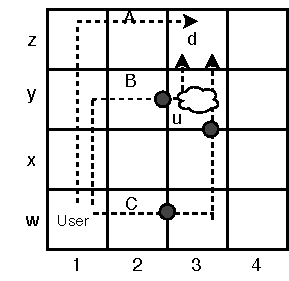
\includegraphics[width=0.7\columnwidth]{single.pdf}}
         \vspace{0.1mm}
        \caption{An example of helpful intervention.}
        \label{fig:single}
\end{figure}


%=========================================================================
%=========================================================================
%=== problem
%=========================================================================
%=========================================================================

\section{Intervention as Planning}
\label{sec:intervention}

We develop an approach whereby plans leading to $\mathrm{u}$ or $\mathrm{d}$ are identified using the recognition approach advanced by Ramirez and Geffner (2009, 2010).
The observer should allow the user to pursue plans leading to $\mathrm{d}$ and intervene when the user takes actions from plans that get ``too close'' to $\mathrm{u}$.
Our key insight is considering $\mathrm{u}$ as a ``goal'', which is justified for planning where we want to identify plan suffixes that lead to undesirable outcomes. 
Undesirable plans $\Pi_{\mathrm{u}}$ are plans that achieve $\mathrm{u}$ and desirable plans $\Pi_{\mathrm{d}}$ achieve $\mathrm{d}$. 
Thus, the observer must consider the two states together $\mathcal{G}=\lbrace\mathrm{u} \cup \mathrm{d}\rbrace$
The observer's recognition problem is: in domain $D$, given $O = \lbrace o_1, \ldots o_{i-1}\rbrace$, what is the most likely ``goal'' from $\mathcal{G}$ if $o_i$ will be observed? 
When $\mathrm{u}$ and $\mathrm{d}$ are far apart, intervention is straightforward; when they are proximate, the observer may find it difficult to recognize $\mathrm{u}$. 


Identifying critical actions requires that the observer consider all potential sources of damage to the user's planning problem, regardless the initial likelihood.
In intervention, the observer asks the question: in domain $D$, given $O = \lbrace o_1, \ldots o_{i-1}\rbrace$ must $o_i \in O$ be flagged to prevent reaching $\mathrm{u}$ first?
%\debug{mak}{perhaps move these assumptions to the list of assumptions below?}
The observer makes this decision while observations arrive incrementally. 
If we are to solve intervention as a plan recognition problem, we need to assume a prior probability distribution (e.g., uniform) over $\mathcal{G}$. However, assuming the distribution of $Pr$ is less reasonable because from the user's perspective, $\mathrm{d}$ is more likely while $\mathrm{u}$ is not. 


\theoremstyle{definition}
\begin{definition}
The \textnormal{online plan intervention problem} is a tuple $\mathcal{I} = \langle D, O, \mathcal{G} \rangle$ where $D=\langle F, A, I \rangle$ is a planning domain, 
$O$ is  sequence of observed actions, $\mathrm{d},\mathrm{u} \in \mathcal{G}$ and 
$\mathrm{d}, \mathrm{u} \subseteq F$
\end{definition}
The user solves the planning problem $P_0=\langle F_0, A_0, I_0,\mathrm{d}\rangle$, where $F_0 \subset F$, $A_0\subseteq A$, $I_0 \subseteq I$ and $\mathrm{d}\subset F$. 
Because $\mathrm{u}\subset F$, $\mathrm{u}\neq \mathrm{d}$ and $\mathrm{u}$ is hidden to the user, some solutions to $P_0$ become undesirable.
Observations for $\mathcal{I}$, has actions from $\Pi_{\mathrm{u}}$ and $\Pi_{\mathrm{d}}$. 

A solution to $\mathcal{I}$ is a sequence of binary decisions that maps the observations $o_i\in O$ to $\lbrace Yes,No\rbrace$ indicating whether the observation requires intervention. 
We discuss two methods to derive functions that perform the mapping. 
The first method uses a data structure called an \textit{Intervention Graph}. 
The second method apply machine learning algorithms using features sampled from the plan space of the observer's recognition problem.
At the very latest, the observer must flag actions having post-conditions such that, if added make $\mathrm{u}$ true (e.g., \texttt{move y2 y3} in Figure~\ref{fig:single}). 
These two conditions (late vs. early) require different decision functions. 
In this paper, we discuss the design of the decision function $\mathcal{F}$ that flags the latest (i.e., most critical) actions. Therefore, we define the critical action to only reflect what it means to be \textit{late}.
\begin{definition}
A \textnormal{late critical action} $a_{crit} \in O$ is an action that occurs in any undesirable plan $\pi_{\mathrm{u}}\in \Pi_{\mathrm{u}}$ and execution of $a_{crit}$ in state $s$ results in a state $s^\prime$ such that $s^\prime\models \mathrm{u}$.
\end{definition}
\noindent There may be more than one $a_{crit}$ in $O$ for the user's planning problem $P_0$. So, the key decision for the observer is whether to intervene when $a_{crit}$ is observed. For this we use the intervention decision function $\mathcal{F}$
\begin{definition}
An \textnormal{intervention decision function} $\mathcal{F}$ takes as input, example actions (of a critical level $\Theta$) in a number of $P_0$ planning problem instances and a set of domain independent features (described next) corresponding to those critical actions and produces a learned model that can recognize actions of the same critical level $\Theta$ occurring in observations of a new planning instance.
\end{definition}
\noindent$\Theta\mapsto\lbrace$`late',`early'$\rbrace$ is an application specific constant.

%=========================================================================
%=========================================================================
%===  example
%=========================================================================
%=========================================================================
\section{Intervention With a ``Competitor''}
\label{sec:example}
Above, we introduced the simple version of the intervention problem.
But sometimes there is another agent interacting with the environment at the same time as the user.
We introduce an additional actor, the \textit{competitor}. 
The competitor is not a standard adversary like you would find in a two-player game.
The competitor has a limited set of actions, which he uses to create states that will lead to $\mathrm{u}$ before $\mathrm{d}$ is reached. 

Figure \ref{fig:multi} shows examples with the competitor in a modified version of the block-words domain used in \cite{ramirez2009plan}.
Figure \ref{fig:multi} (top) shows a problem with 4 blocks (T, B, A, D) initially on the table and time flows from left to right. 
$\mathrm{d}=$ (TAD) and $\mathrm{u}=$ (BAD).
The user does not know about the competitor's modifying the state of block B (dotted line block) nor about $\mathrm{u}$.
Thus the user may enable $\mathrm{d}$ with the action \texttt{stack (user,A,D)} and at the same time creating an opportunity for the competitor to reach $\mathrm{u}$ first. 
Assuming the user and the competitor are optimal in this example, if the observer is intervening late ($\Theta=late$), $a_{crit}=\lbrace$\texttt{stack(competitor,B,A)}$\rbrace$. 


When intervening early ($\Theta=early$), we define a critical sequence $s_{crit}$ that the observer must flag.
\begin{definition}
A \textnormal{critical sequence} $s_{crit} \subseteq O$ is a totally ordered set of actions in any undesirable plan $\pi_{\mathrm{u}}\in \Pi_{\mathrm{u}}$ and ordered execution of actions in $s_{crit}$ from state $s$ results in a state $s^\prime$ such that $s^\prime\models \mathrm{u}$.
\end{definition}
\noindent In Figure \ref{fig:multi} (top), $s_{crit}=\lbrace$\texttt{pickup(competitor,B)}, \texttt{stack(competitor,B,A)}$\rbrace$.
Figure \ref{fig:multi}~(bottom) shows a problem with a longer $s_{crit}$.
Here, $\mathrm{d}= $ (CUP) and $\mathrm{u}= $ (CUT), the user does not observe block T, 
and intervention must happen when \texttt{STACK(competitor, T, P)} is observed. If not, the user could unwittingly reach $\mathrm{u}$ by placing U on T (thinking P is free) and stacking C on U. 
Thus, any subsequent action leading  to $\mathrm{u}$ must also be flagged to prevent the error. 
Therefore, $s_{crit}=\lbrace$\texttt{stack(competitor,T,P)}, \texttt{pickup(user,U)},\texttt{stack(user,U,T)}, \texttt{pickup(user,C)},\texttt{stack(user,C,U)}$\rbrace$.

\begin{figure}[t]
          \centering{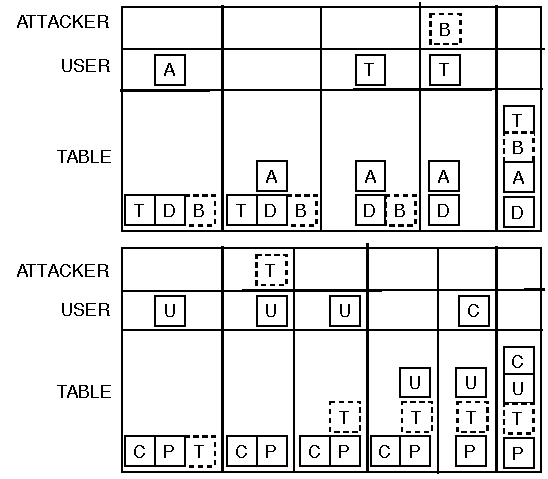
\includegraphics[width=0.7\columnwidth]{bw.pdf}}
        \caption{Reaching $\mathrm{u}= $ (BAD) (top) and $\mathrm{u}= $ (CUT) (bottom) with an competitor and a user.  The table initially contains all four blocks in each example. A block in the user or competitor row indicates a pickup action that is removed using a stack action.}
        \label{fig:multi}
\end{figure}

%\debug{mak}{provide a new definition for this variant of the problem}
\begin{definition}
The \textnormal{online plan intervention problem} with a competitor is a tuple $\mathcal{I} = \langle D, O, \mathcal{G} \rangle$ where $D=\langle F_0\cup F_1, A_0\cup A_1, I \rangle$ is a planning domain, 
$O$ is  sequence of observed actions, $\mathrm{d},\mathrm{u} \in \mathcal{G}$ and 
$\mathrm{d}, \mathrm{u} \subseteq F_0\cup F_1$
\end{definition}
The user solves the planning problem $P_0=\langle F_0, A_0, I,\mathrm{d}\rangle$.
The competitor wants to solve the planning problem $P_1=\langle F_1, A_1, I,\mathrm{u}\rangle$.
However, the competitor does not have access to all the actions needed to achieve $\mathrm{u}$ and requires the user to enable preconditions for the actions in $A_1$ and $A_1 \cap A_0=\emptyset$ and $F_1 \neq F_0$. This and because $\mathrm{u}$ is hidden to the user, some solutions to $P_0$ become undesirable.
Observations for $\mathcal{I}$, contain actions from $A_0$ and $A_1$.
For example, in Figure \ref{fig:multi}(top), the competitor can only perform actions with the hidden block (stack B, pickup B etc.), and the user can not recognize effects of these \textit{hidden} actions. 

The execution model of the agents is such that the user and the competitor (if present) take turns in proposing actions to the observer. Which agent proposes first is decided randomly. Given an observation trace $O = \lbrace o_1, o_2,\ldots o_{i-1}\rbrace$, the observer sees the effects of the actions upto $o_{i-1}$. The user or the competitor (if present) proposes the next action $a_i$ to execute from their respective action sets $A_0$ and $A_1$. The proposed action becomes the observation $o_i$ only if it's approved (i.e., action does not need intervention).

In this study, we make several assumptions about the observer.
\textbf{(Observability)} 
The observer has full observability, knows about both $\mathrm{d}$ and $\mathrm{u}$ and helps the user avoid $\mathrm{u}$ by flagging critical actions.
\textbf{(Plans)} 
The user follows a satisficing plan to reach $\mathrm{d}$, but may reach the hidden $\mathrm{u}$ unwittingly. 
There is a satisficing plan to reach $\mathrm{u}$ and we assume that it has a common prefix with a plan to reach $\mathrm{d}$. 
Throughout execution, the user sticks to his original plan; and do not replan. System execution stops when either $\mathrm{u}$ or $\mathrm{d}$ is reached first.
\textbf{(Competitor)}
When present, the competitor only perform actions using objects hidden to the user; this restriction follows from many security domains where an attacker is a remote entity that plants traps and expects the user to become an unwitting accomplice (e.g., attacker sends click-bait phishing email to the user and expects the user to click the link, without doing anything else on the user's computer).





\section{The Intervention Graph}
\label{sec:stategraph}
We define the intervention graph, which models the decision space of the observer.
We then extract several features from the  intervention graph, which we use to define $\mathcal{F}$.
Unfortunately, extracting these features can be intractable when the intervention graph is large, as can happen with with larger problems, multiple paths reaching $\mathrm{d}$, or multiple undesirable goals. Therefore, we define an additional set of features by sampling the plan space, where the samples are obtained with the Top-K planner \cite{riabov2014}.

The Intervention Graph allows the intervening agent to evaluate how close in the state space the current projection of the observed partial plan is to $\mathrm{u}$. The Intervention Graph consists of alternating state and action layers where each state layer consists of predicates that have been made true by the actions in the previous layer. An action layer consists of actions $a\in A$ whose preconditions are satisfied in the state. Algorithm \ref{bsg} describes the process of building the Intervention Graph. The algorithm takes as input a domain theory $D$, state $s$ and $\mathcal{G}=\lbrace\mathrm{u},\mathrm{d}\rbrace$ (lines 1-2). Before any observations have been made, the current state (i.e., root of the tree) is set to initial state $I$. Next, using the domain theory $D$, actions  $a\in A$ whose preconditions are satisfied at current state are added to the graph (lines 5-6). Each action in level $i$ spawns possible states for level $i+1$. Line 7 ensures that backtrack actions are not added to the graph. This is because the user and the competitor (if present) in our domain are (bounded) rational agents and their respective action sets ($A_0$, $A_1$) are disjoint. For each applicable effect state a search vertex is created, with an edge, representing the action responsible for the state transition connecting the parent and the child (lines 8-10). Calling the method recursively for each state until $\mathrm{d}$ and $\mathrm{u}$ are added to some subsequent level in the graph will generate a possible hypotheses space for the observer (line 11). To ensure that only realistic plans are explored, we do not add no-op actions to the action layers in the graph. As a new observation arrives, the root of the graph is changed to reflect the new state after the observation and subsequent layers are also modified to that effect.  
%\debug{mak}{clarify how the IG is different from the actual RPG and discuss algorithm in detail. Alternatively, consider forgoing the link to the RPG and just discussing the IG in terms of the search space. }
%\debug{sachini}{why does the IG need to explore longer plans that those that reach $G_d$.  Mak: Explore around the fringe because we don't know where $\mathrm{u}$ ``lives.''}
\begin{algorithm}[tb]
%\scriptsize
        \caption{Build Intervention Graph}
        \label{bsg}
        \begin{algorithmic}[1]
                \Require $D$, $s$, $\mathcal{G}$
                \State $i=0;$ $ s_{i} \gets I $
                \Procedure{expandgraph}{$D,s,\mathcal{G}$}
                \If{$s_{i} \models \mathrm{u},\mathrm{d}$} return $\langle V,E\rangle$
                \Else
                        \For{$a \in A$ where $Pre(a) \in s_{i}$}
                                \State \parbox[t]{0.95\linewidth} 
                                {$s_{i+1} \gets ((s_{i} \setminus Del(a))\cup Add(a))$}
                                \If{$s_{i+1} \equiv s_{i}$} continue \EndIf
                                \State $v \gets$ AddVertex ($s_{i+1}$)
                                \State $e \gets$ AddEdge ($s, s_{i+1}, a$)
                                \State $V \cup \{v\}$ $; E \cup \{e\}$
                                \State ExpandGraph ($D, s_{i+1}, \mathcal{G}$)
                        \EndFor
                \EndIf  
                \EndProcedure
        \end{algorithmic}
\end{algorithm}

Thus, the Intervention Graph is a weighted, single-root, directed acyclic connected graph $IG= \langle V,E \rangle$, where $V$ is the set of vertices denoting possible states the user could be in until $\mathrm{d}$ is reached, and $E$ is the set of edges representing actions from $A_0 \cup A_{1}$. A path from the root of the tree to $\mathrm{d}$ that goes through $\mathrm{u}$ represents an undesirable plan, while a path from root to a node containing $\mathrm{d}$ that bypasses $\mathrm{u}$ represents a desirable plan. The Intervention Graph is also helpful in separating truly unsafe situations from states where the user can tolerate the competitor's actions (e.g., nuisances) and still reach $\mathrm{d}$ by bypassing $\mathrm{u}$. 

%add if find space
%\textbf{Example:} Figure \ref{fig:fails} extends the example from Figure \ref{fig:multi} (A). Because block B is invisible, the user accepts all the four formations as successfully reaching $\mathrm{d}$. However, case (2) is a truly unsafe situation because the user has unwittingly reached $\mathrm{u}$. The observer must be able to flag a correct $a_{crit}$ case (2). In contrast, plans leading to the states shown in cases (1), (3) and (4) should be identified as safe by the observer, because $\mathrm{u}$ is not achieved. Actions in these plans must not be flagged as critical.
%\begin{figure}[ht]
%        \centering{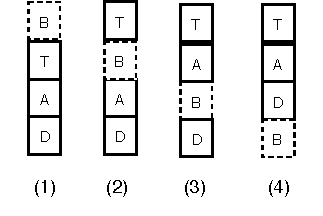
\includegraphics[width=0.6\columnwidth]{activefail.pdf}}
%        \caption{User's attempts to reach $\mathrm{d}$ in the presence of competitor}
%        \label{fig:fails}
%\end{figure}


\section{Extracting Features From The Intervention Graph}
\label{sec:features}
We extract a set of features from the intervention graph that help determine when to intervene. These features include: Risk, Desirability, Distance to $\mathrm{d}$, Distance to $\mathrm{u}$ and Percentage of active undesirable landmarks in current state. We use these features to train a classifier that learns to identify $a_{crit}$. Figure \ref{fig:feature} illustrates a fragment of the intervention graph from Figure \ref{fig:multi} (A) after observing \texttt{PICK-UP A}, which we will use as a running example to discuss feature computation.

\begin{figure*}[tb]
        \centering{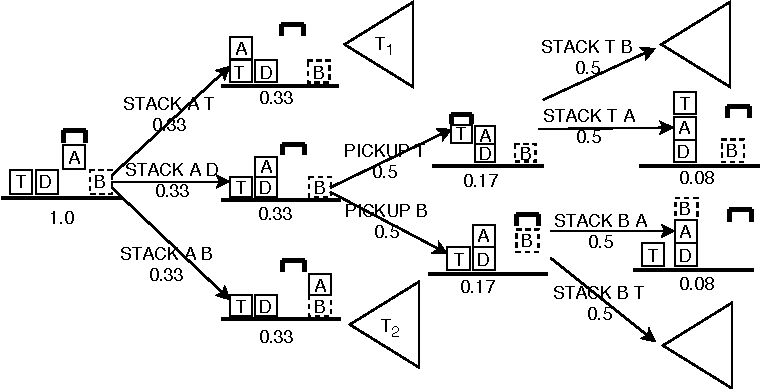
\includegraphics[width=0.75\textwidth]{features.pdf}}
        \caption{Fragment of the decision space after PICKUP A has been observed for block-words example in Figure \ref{fig:multi} (A). Numbers under each state and action indicate the probability. Sub trees $T_1$ and $T_2$ are not expanded for simplicity.}
        \label{fig:feature}
\end{figure*} 

\textbf{Risk ($R$)} quantifies how likely the effects of current observation will lead to $\mathrm{u}$. $R$ is also coupled with the uncertainty the observer has about the next observation. We model the uncertainty as a uniform probability distribution across the set of actions whose preconditions are satisfied in current state. We define $R$ as the posterior probability of reaching $\mathrm{u}$ while the user is trying to achieve $\mathrm{d}$. Given the intervention graph, we extract paths from root to any leaf containing the $\mathrm{d}$, including the ones in which the user has been subverted to reach $\mathrm{u}$ instead. By virtue of construction termination, $\mathrm{d}$ will always be a leaf.
Let $\Pi_{\mathcal{C}}$ be the candidate plans reaching $\mathrm{d}$ and let $\left | \Pi_{\mathcal{C}} \right |=n$. The plan set $\Pi_{u}$ contains action sequences that reach state $\mathrm{u}$ such that, $\Pi_{u} \subseteq \Pi_{\mathcal{C}}$, $\left | \Pi_{u} \right |=m$ and $(m<=n)$. We compute posterior probability of reaching $\mathrm{u}$ for a path $\pi \in \Pi_{u}$, using chain rule in probability as, $P_{\pi}=\prod_{j=1}^{k}P(\alpha_j|\alpha_1, \alpha_2,...,\alpha_{k-1})$, and $\alpha_{j} \in A$ and $k$ is the length of path until $\mathrm{u}$ is reached. Then: 
\begin{equation*} 
R = \left\{\begin{matrix} \frac{\sum_{i=1}^{m}P_{\pi_i}}{m} & m>0\\ 0 &  m=0 \end{matrix}\right.
\end{equation*}
According to example in Figure \ref{fig:feature}, $(n=6)$ and $(m=1)$. Since we assumed full observability for the observer, the root of the tree (current state) is assigned the probability of 1.0. Then, actions that are immediately possible after current state are each assigned probabilities following a uniform distribution across the branching factor (0.33). Then for each applicable action in the current state, the resulting state gets the probability of ($1.0\times0.33=0.33$). Similarly, we apply the chain rule of probability for each following state and action level in the graph until $\mathrm{u}$ first appears in the path. $R=\frac{0.08}{1}=0.08$.

\textbf{Desirability ($D$)} measures the effect of the observed action to help the user pursue the desirable goal safely. Given $\Pi_{\mathcal{C}}$ as the set of plans extracted from the intervention graph that reach $\mathrm{d}$ and $\left | \Pi_{\mathcal{C}} \right |=n$. The plan set $\Pi_{d}$ contains action sequences that reach state $\mathrm{d}$ without reaching $\mathrm{u}$, $\Pi_{d} = \Pi_{\mathcal{C}} \setminus \Pi_{u} $, we compute  posterior probability of reaching $\mathrm{d}$ without reaching $\mathrm{u}$ for a path $\pi \in \Pi_{d}$, using chain rule in probability as, $P_{\pi}=\prod_{j=1}^{k}P(\alpha_j|\alpha_1, \alpha_2,...,\alpha_{k-1})$, and $\alpha_{j} \in A$ and $k$ is the length of path. Then:
\begin{equation*} 
D = \left\{\begin{matrix}
\frac{\sum_{i=1}^{n-m}P_{\pi_i}}{n-m} & n-m>0\\ 
0 &  n-m=0
\end{matrix}\right.
\end{equation*} 
In Figure \ref{fig:feature}, there are five instances where user achieved $\mathrm{d}$  without reaching $\mathrm{u}$ (two in sub tree $T_1$, three in the expanded branch). Following the same approach to assign probabilities for states and actions, $D= \frac{(0.08+0.08+0.08+0.04+0.04)}{5} = 0.07$.
$R$ and $D$ are based on probabilities indicating the confidence the observer has about the next observation. We also use simple distance measures: (1) distance to $\mathrm{u}$  ($\delta_u$) and (2) distance to $\mathrm{d}$ ($\delta_d$). Both distances are measured in the number of actions required to reach a state containing $\mathrm{d}$ or $\mathrm{u}$ from root in the intervention graph.  

\textbf{Distance to $\boldsymbol{\mathrm{u}}$} ($\delta_u$) measures the distance to state $\mathrm{u}$ from the current state in terms of the number of actions. As with the computations of $R$ and $D$, given $\Pi_{\mathcal{C}}$ is the set of paths extracted from the intervention graph that reach $\mathrm{d}$ and $\left | \Pi_{\mathcal{C}} \right |=n$. The path set $\Pi_{u}$ contains action sequences that reach state $\mathrm{u}$ such that, $\Pi_{u} \subseteq \Pi_{\mathcal{C}}$, $\left | \Pi_{u} \right |=m$ and $(m<=n)$. We count  $s$, the number of the edges (actions) before $\mathrm{u}$ is reached for each path $\pi \in \Pi_{u}$ and $\delta_u$ is defined as the average of the distance values given by the formula:
\begin{equation*} 
\delta_u = \left\{\begin{matrix}
\frac{\sum_{i=1}^{m}s_i}{m} & m>0\\ 
-1 &  m=0
\end{matrix}\right.
\end{equation*} 
In this formula, $-1$ indicates that the undesirable state is not reachable from the current state. For the example problem illustrated in Figure \ref{fig:feature}, $\delta_u=\frac{3}{1}=3$. 

\textbf{Distance to $\boldsymbol{\mathrm{d}}$} ($\delta_d$) measures the distance to $\mathrm{d}$ from current state. The path set $\Pi_{d}$ contains action sequences that reach $\mathrm{d}$ without reaching $\mathrm{u}$, $\Pi_{d} = \Pi_{\mathcal{C}} \setminus \Pi_{u} $, we count  $t$, the number of the edges where $\mathrm{d}$ is achieved without reaching $\mathrm{u}$ for each path $\pi \in \Pi_{d}$. Then, $\delta_d$ is defined as the average of the distances given by the formula:
\begin{equation*} 
\delta_d = \left\{\begin{matrix}
\frac{\sum_{i=1}^{n-m}t_i}{n-m} & n-m>0\\ 
-1 &  n-m=0
\end{matrix}\right.
\end{equation*}
In this formula, $-1$ indicates that $\mathrm{d}$ can not be reached safely from the current state. For the example problem illustrated in Figure \ref{fig:feature}, $\delta_d=\left \lceil \frac{3+3+7+7+3}{5} \right \rceil=5$.
%\debug{mak}{integrate the following}


We also use the definition for landmarks by Hoffman et al. \shortcite{hoffman2004lm}, which are propositions that have to be true at some time in every solution plan in a planning problem. Formally: a fact $L_P \subset F$ of a planning task $ P = \langle F, A, I, G \rangle$ is a \textbf{fact landmark} for $P$ iff $L_P$ is true in some state in all valid plans that modifies $I$ to $G$.

\textbf{Percentage of active attack landmarks} ($\mathcal{L}_{ac}$) captures the criticality of current state toward contributing to $\mathrm{u}$. 
Landmarks \cite{hoffman2004lm} are predicates (or actions) that must be true in every valid plan for a planning problem. We used the algorithm in Hoffmann et al. \shortcite{hoffman2004lm} to extract fact landmarks for the planning problem $P = \langle D, \mathrm{u}\rangle$. These landmarks are referred to as attack landmarks ($\mathcal{L}_{u}$) because they establish predicates that must be true to reach $\mathrm{u}$.  Landmarks have been successfully used in deriving heuristics in plan recognition \cite{vered2018goalrec} and generating alternative plans \cite{bryce2014diverse}. We compute a feature using attack landmarks: percentage of active attack landmarks in current state ($\mathcal{L}_{ac}$). To compute $\mathcal{L}_{ac}$ for the example in Figure \ref{fig:feature}, we count the number of landmark predicates that have become active $(l)$ in the root of the intervention graph. Then, ($\mathcal{L}_{ac}$) is given by the formula: $\mathcal{L}_{ac} = \frac{l}{\left |\mathcal{L}_{u}\right|}$. In Figure \ref{fig:feature}, $l=4$ and $\mathcal{L}_{ac}=4/10=0.4$.

Algorithm~\ref{alg:exact} shows the computation of the feature values for a given observation using the intervention graph. The algorithm takes a PDDL domain, a set of undesirable and desirable states as input and produces a relation $\mathcal{V}$ of observations and corresponding feature values. Landmarks for the problem $P = \langle D, \mathrm{u}\rangle$ are computed apriori (line 3). Then, as observations are revealed incrementally, the intervention graph is generated and the feature set is computed (lines 4-11). Finally, the state is updated to reflect the effect of the most recent observation (line 12).

\section{Sampling the Intervention Graph and Using Sampled Features}
To overcome the state space explosion while building the graph in large domains like the Rush Hour puzzle \cite{fernau2003}, we propose a second method. Instead of sampling plans from the full search space, the observer samples only a subset of plans to compute a new feature vector called Sampled Features.
Risk and Desirability allow the observer to assess the likelihood the user will reach $\mathrm{d}$ safely. For example, when there is no alternative path for the user to reach $\mathrm{d}$ by avoiding $\mathrm{u}$ from the current state, Risk value will be high. However, these are intractable to compute in large problems. So we estimate them with plan distance measures. The intuition is that if the user is executing an unsafe plan (high risk), then the reference plan that is compatible with observations will be more similar to a sample of unsafe plans, compared to a sample of safe plans. We use action set distance, state sequence distance, causal link distance \cite{nguyen2012generating}, Generalized Edit Similarity (GED) for sequences of states and actions \cite{sohrabi2016finding} from the plan diversity literature as replacements for Risk and Desirability. We also use Landmark-Based Goal Completion Heuristic \cite{pereira2017} and number of actions to $\mathrm{u}$ and $\mathrm{d}$ as additional features.

The observer computes plan distances between a reference plan ($\pi^\prime$) and sampled plans ($\Pi^{\prime\prime}$) for both $\mathrm{u}$ and $\mathrm{d}$ for each incrementally revealed observation. We borrow from plan/goal recognition to produce $\pi^\prime$ and $\Pi^{\prime\prime}$ that agree with the observation history ($O$). Ramirez and Geffener \shortcite{ramirez2009plan} proposed an approach to compile the observations into the domain theory. Vered et al. \shortcite{vered2016mirror} proposed goal mirroring that concatenates a plan prefix, which agrees with the observations to a plan suffix, which is a plan generated from the last observed point in the prefix to the goal, that can be applied to both continuous and discrete domains. We follow the method proposed by Vered et al. \shortcite{vered2016mirror} in this work to generate observation compatible plans. We concatenate observation history with the optimal plan that reaches $\mathrm{u}$ (and $\mathrm{d}$) to produce $\pi^\prime$. Generating observation compatible $\pi^\prime$ and $\Pi^{\prime\prime}$ by compiling the observations into the domain theory is a possible extension to this work, which will be explored in the future. We use the Top-K planner with K$=$50 \cite{riabov2014}, to sample the plan space. Algorithm \ref{alg:apx} computes the feature vector from sampling the plan space. For action, state sequence and causal link distances we use the median of all $\langle$reference, sample$\rangle$ plan pairs as the feature value. We use the minimum distance to goal state for all $\langle$reference, sample $\rangle$ pairs. For action and state GED, we use the minimum for all $\langle$reference, sample$\rangle$ pairs.
\vspace{-2mm}
\begin{algorithm}[tb]
%\scriptsize
        \caption{Build Full Vectors}
        \label{alg:exact}
        \begin{algorithmic}[1]
                \Require $D$, $I$, $O$, $\mathrm{u}$, $\mathrm{d}$.
                \Procedure{Full}{$D,O,I,\mathrm{u},\mathrm{d}$}
                \State $i=0;$ $ s_i \gets I$
                \State $\mathcal{L}_{u} \gets$ compute remaining landmarks for the problem $P_\alpha=\langle D_\alpha, \mathrm{u}\rangle$
                \For{$o \in O$}
                        \State $G(V,E) \gets ExpandGraph(D,s_i,\mathrm{u},\mathrm{d})$
                        \State $R_o \gets$ compute $Risk$ using $IG$
                        \State $D_o \gets$ compute $Desirability$ using $IG$
                        \State $\delta_{u_o} \gets$ compute mean distance to critical state using $IG$
                        \State $\delta_{d_o} \gets$ compute mean distance to desirable state using $IG$
                        \State $\mathcal{L}_{{ac}_o} \gets$ active landmark \% using $s_i$ and  $\mathcal{L}_{u}$
                        \State $\mathcal{V}(o) \gets \lbrack R_o,D_o,\delta_{u_o}, \delta_{d_o}, \mathcal{L}_{{ac}_o}\rbrack$
                        \State {$s_{i+1} \gets ((s_{i} \setminus Del(o))\cup Add(o))$}
                \EndFor
                \EndProcedure
        \end{algorithmic}
\end{algorithm}
\setlength{\textfloatsep}{2pt}
\begin{algorithm}[tb]
%\scriptsize
        \caption{Build Sampled Vector}
        \label{alg:apx}
        \begin{algorithmic}[1]
                \Require $D$, $s$, $\mathrm{u}$, $\mathrm{d}$
                \State $i=0;$ $ s_{i} \gets I $
                \State $prefix,suffix,\Pi^{\prime\prime}, \mathcal{V} \gets \varnothing$
                \Procedure{Partial}{$D,s,\mathrm{u},\mathrm{d},O$}
                        \State $\mathcal{L}_{u} \gets$ compute remaining landmarks for the problem $P_\alpha=\langle D_\alpha, \mathrm{u}\rangle$
                \For{$o \in O$}
                        \State \parbox[t]{0.95\linewidth}{$prefix \gets prefix + o$}
                        \State \parbox[t]{0.95\linewidth} 
                                {$s_{i+1} \gets ((s_{i} \setminus Del(o))\cup Add(o))$}
                        \For {$ g \in \{\mathrm{u}, \mathrm{d}$\}}
                                \State \parbox[t]{0.95\linewidth}{$suffix \gets OptimalPlan(s,g)$}
                                \State \parbox[t]{0.95\linewidth}{$\Pi^\prime \gets prefix + suffix$}
                                \State \parbox[t]{0.95\linewidth}{$\Pi^{\prime\prime} \gets \text{Observation compatible Top-K plans for } g$}
                                \State \parbox[t]{0.95\linewidth}{$v_1 \gets$ MedianActionSetDist$(\Pi^\prime, \Pi^{\prime\prime})$}
                                \State \parbox[t]{0.95\linewidth}{$v_2 \gets$ MedianCausalLinkDist$(\Pi^\prime, \Pi^{\prime\prime})$}
                                \State \parbox[t]{0.95\linewidth}{$v_3 \gets$ MedianStateSequenceDist$(\Pi^\prime,\Pi^{\prime\prime})$}
                                \State \parbox[t]{0.95\linewidth}{$v_4 \gets$ MinimumDistToState $(g,\Pi^{\prime\prime})$}
                                \State \parbox[t]{0.95\linewidth}{$v_5 \gets$ MinimumActionGED $(\Pi^\prime, \Pi^{\prime\prime})$}
                                \State \parbox[t]{0.95\linewidth}{$v_6 \gets$ MinimumStateGED $(\Pi^\prime, \Pi^{\prime\prime})$}
                                \State $\mathcal{V}(o) \gets \lbrack v_1,v_2,v_3,v_4,v_5,v_6\rbrack $
                        \EndFor
                        \State \parbox[t]{0.95\linewidth}{$v_7 \gets$ AchievedLandmarkHeuristic $(\mathrm{u},s_{i})$}
                        \State $\mathcal{V}(o) \gets \mathcal{V}(o)+\{v_7\}$
                \EndFor
                \EndProcedure
        \end{algorithmic}
\end{algorithm}

%=========================================================================
%=========================================================================
%=== algorithm
%=========================================================================
%=========================================================================
\section{Learning When to Intervene}
The observer is learning to generate alerts when detecting $a_{crit}$ while the user is in a goal-oriented but unsafe path. %It may be possible to equip planners to produce plans, avoiding the undesirable states while optimizing for metrics like plan length so that the observer can produce ``safe'' plans on user's behalf.
We train a classifier in supervised learning mode to categorize observed actions into two classes: (Y) indicating interruption is warranted and (N), indicating otherwise. According to this policy, for the blocks-words example in Figure \ref{fig:multi} (A), the following observation sequence labeled as: PICK-UP A (N), STACK A D (N), PICK-UP B (N), STACK B A (Y), PICK-UP T (Y). In this observation sequence $a_{crit}=$STACK B A. Given a labeled observation set and corresponding feature vectors, we train the classifiers with 10-fold cross validation. Then the trained model is used to predict intervention for previously unseen, new intervention problems. We chose attribute selected Naive Bayes, K-nearest neighbors, decision tree and logistic regression classifiers from Weka~\footnote{\url{http://www.cs.waikato.ac.nz/ml/weka/}}. Attribute selected classifiers filter the feature vector to only select critical features. This step reduces complexity of the model, makes the outcome of the model easier to interpret, and reduces over-fitting. To generate training data we first created twenty intervention problems for the benchmark domains and the new Rush Hour domain and enforced a limit of 100 observation traces per problem. We selected these classifiers because they are commonly used interpretable models, which we hope to utilize in generating explanations for intervention in future work.

%While there are many model-agnostic methods for explaining predictions for classifiers (e.g., LIME \cite{ribeiro2016}, Shapely values), for simplicity we opted to adopt commonly used interpretable models to learn when to intervene. Additionally, we want to draw focus toward explaining event causality associated with the undesirable state (i.e., what events caused intervention). Associations learned by the supervised learning algorithms do not reflect event causality.
%For each classifier we select parameters to tune and compared their effect on the model accuracy for both benchmark and Rush Hour domains. For the decision tree, we tuned pruning confidence (C) and minimum number of instances per leaf (M). For the K-nearest neighbor classifier we tune K and the distance metric (dis). Naive Bayes classifier is tuned with the supervised discretization parameter (D). The logistic regression classifier was tuned with the ridge parameter (R).
 
A full parameter search revealed the best parameters for the classifiers. The decision tree classifier is tuned to pruning confidence=0.25 and minimum number of instance per leaf=2. K-nearest neighbor classifier is tuned to use k=1 and distance measure=Euclidean. Logistic regression classifier is tuned for ridge parameter = 1.0E-8. Naive Bayes classifier is tuned with the supervised discretization=True. For the intervention graph approach, the learned models chose distance to $\mathrm{u}$ and Risk as the dominant features for the benchmark domains. We were not able to identify clear dominant features in feature vectors built with plan space sampling.

%ran experiments using the Weka workbench to evaluate classifier accuracy (dependent variable) to varying parameter for the classifiers (independent variables). Table \ref{tab:tuned} summarizes results, with boldface values indicating the selected parameter values that produced best accuracy (95\% confidence interval) for all the domains.
%\begin{table}[ht]
%\small
%\begin{tabular}{|l|l|}
%\hline
%\multicolumn{1}{|c|}{Classifier} & \multicolumn{1}{c|}{Tested Values}                                                        \\ \hline
%Decision tree                    & \begin{tabular}[c]{@{}l@{}}C = {[}0.05,0.1,\textbf{0.25},0.5{]}\\ M = {[}\textbf{2},5,10{]}\end{tabular}    \\ \hline
%K-nearest neighbor               & \begin{tabular}[c]{@{}l@{}}K = {[}\textbf{1},3,7{]}\\ Dis = {[}\textbf{Eucledean},Manhattan{]}\end{tabular} \\ \hline
%Naive Bayes                      & D = {[}\textbf{True},False{]}                                                                      \\ \hline
%Logistic regression              & R = {[}1.0E-2,1.0E-4,\textbf{1.0E-8},1.0E-16{]}                                                    \\ \hline
%\end{tabular}
%\caption{Parameter tuning for intervention classifiers}
%\label{tab:tuned}
%\end{table}
% 
 
%=========================================================================
%=========================================================================
%=== results
%=========================================================================
%=========================================================================
\section{Results and Discussion}
We focus on two questions: (1) Using domain-independent features indicative of the likelihood to reach $\mathrm{u}$ from current state, can the observer correctly interrupt to prevent the user from reaching $\mathrm{u}$? and (2) How does the learning approach perform against state-of the-art goal recognition? To address the first question, we evaluated the performance of the learned model to predict intervention on previously unseen problems.

The benchmark suite consists of Blocks-words, IPC Grid, Navigator and Ferry domains and the Generalized Rush Hour domain. For the \textbf{Blocks-words} domain, we chose word building problems. The words user and the competitor want to build are different but they have some common letters (e.g., TAD/BAD). The competitor is able to exploit the user's progress on stacking blocks to complete word the competitor wants to build and uses a hidden block in the domain to create nuisance scenarios. In the \textbf{IPC grid} domain, the user agent moves through a grid to get from point A to B. Certain locked positions on the grid can be opened by picking up keys. In the \textbf{Navigator} domain, the user agent simply moves from one point in grid to another. In Easy-IPC and Navigator domains, we designated certain locations on the grid as traps. The goal of the user is to navigate to a specific point on the grid safely. In the \textbf{Ferry} domain, a single ferry (akin to a user) moves cars between different locations. In the Ferry domain a port is \emph{compromised}. The ferry's objective is to transport cars to specified locations without passing the compromised port. In the \textbf{Rush Hour} domain, we created puzzles containing vehicles that need not be moved on arbitrary grid sizes and exits. The player (user agent) wins by moving a designated goal car to the exit. We also designated some vehicles on the grid as forbidden. The forbidden vehicles need not be moved to solve the puzzle. Intervention is generated when the user moves any of the forbidden vehicles while solving the puzzle.

We generate 3 separate test instances of 20 problems each (total of 60) for the benchmark domains containing problems different from trained instances. For example, number of blocks in the domain (block-words), size of grid (navigator, easy-ipc), number of cars and exit locations (Rush Hour), accessible and inaccessible paths on the grid (navigator, easy-ipc), properties of artifacts in the grid (easy-ipc). For each problem in an instance we generated 10 observation traces (total of 600 test observation traces). For the Rush Hour domain we created 2200 observation traces and split to training and testing 60/40. We define true-positive as the classifier correctly predicting $a_{crit}$. True-negative is an instance where the classifier  correctly predicts an observation as not critical. False-positives are instances where classifier incorrectly predicts $a_{crit}$. False-negatives are instances where the classifier incorrectly predicts the observation not as critical. Naturally, our test observation traces contain a large number of negatives. To offset the bias introduced to the classifier by the class imbalance, we report Matthews correlation coefficient (MCC) along with the F1 measure. We report the MCC because, it gives an accurate measure the quality of a binary classification while taking into account the different class sizes. In our data set, there are many negative observations.


\begin{table*}[tb]
\resizebox{\textwidth}{!}{%
\begin{tabular}{|l|llllll|llllll|llllll|llllll|}
\hline
\multicolumn{1}{|c|}{\multirow{3}{*}{Domain}} & \multicolumn{6}{c|}{Naive Bayes}                                                                                                          & \multicolumn{6}{c|}{Decision Tree}                                                                                                      & \multicolumn{6}{c|}{Logistic Regression}                                                                                                & \multicolumn{6}{c|}{K-Nearest}                                                                                                             \\ \cline{2-25} 
\multicolumn{1}{|c|}{}                        & \multicolumn{2}{c|}{Inst 1}                        & \multicolumn{2}{c|}{Inst 2}                        & \multicolumn{2}{c|}{Inst 3}     & \multicolumn{2}{c|}{Inst 1}                        & \multicolumn{2}{c|}{Inst 2}                        & \multicolumn{2}{c|}{Inst 3}   & \multicolumn{2}{c|}{Inst 1}                        & \multicolumn{2}{c|}{Inst 2}                        & \multicolumn{2}{c|}{Inst 3}   & \multicolumn{2}{c|}{Inst 1}                         & \multicolumn{2}{c|}{Inst 2}                         & \multicolumn{2}{c|}{Inst 3}    \\ \cline{2-25} 
\multicolumn{1}{|c|}{}                        & \multicolumn{1}{l|}{F1} & \multicolumn{1}{c|}{MCC} & \multicolumn{1}{c|}{F1} & \multicolumn{1}{l|}{MCC} & \multicolumn{1}{l|}{F1} & MCC   & \multicolumn{1}{l|}{F1} & \multicolumn{1}{l|}{MCC} & \multicolumn{1}{l|}{F1} & \multicolumn{1}{l|}{MCC} & \multicolumn{1}{l|}{F1} & MCC & \multicolumn{1}{l|}{F1} & \multicolumn{1}{l|}{MCC} & \multicolumn{1}{l|}{F1} & \multicolumn{1}{l|}{MCC} & \multicolumn{1}{l|}{F1} & MCC & \multicolumn{1}{l|}{F1} & \multicolumn{1}{l|}{MCC}  & \multicolumn{1}{l|}{F1} & \multicolumn{1}{l|}{MCC}  & \multicolumn{1}{l|}{F1} & MCC  \\ \hline
\multicolumn{25}{|c|}{Intervention Graph Method}                                                                                                                                                                                                                                                                                                                                                                                                                                                                                                                                                                                         \\ \hline
\textbf{Blocks}              & 1                       & \multicolumn{1}{l|}{1}   & 1                       & \multicolumn{1}{l|}{1}   & 1                       & 1     & 1                       & \multicolumn{1}{l|}{1}   & 1                       & \multicolumn{1}{l|}{1}   & 1                       & 1   & 1                       & \multicolumn{1}{l|}{1}   & 1                       & \multicolumn{1}{l|}{1}   & 1                       & 1   & 1                       & \multicolumn{1}{l|}{1}    & 1                       & \multicolumn{1}{l|}{1}    & 1                       & 1    \\ \cline{1-1}
\textbf{EasyIPC}             & 1                       & \multicolumn{1}{l|}{1}   & 1                       & \multicolumn{1}{l|}{1}   & 1                       & 1     & 1                       & \multicolumn{1}{l|}{1}   & 1                       & \multicolumn{1}{l|}{1}   & 1                       & 1   & .88                     & \multicolumn{1}{l|}{.87} & .88                     & \multicolumn{1}{l|}{.87} & .86                     & .86 & 1                       & \multicolumn{1}{l|}{1}    & 1                       & \multicolumn{1}{l|}{1}    & 1                       & 1    \\ \cline{1-1}
\textbf{Ferry}               & 1                       & \multicolumn{1}{l|}{1}   & 1                       & \multicolumn{1}{l|}{1}   & 1                       & 1     & 1                       & \multicolumn{1}{l|}{1}   & 1                       & \multicolumn{1}{l|}{1}   & 1                       & 1   & 1                       & \multicolumn{1}{l|}{1}   & 1                       & \multicolumn{1}{l|}{1}   & 1                       & 1   & 1                       & \multicolumn{1}{l|}{1}    & 1                       & \multicolumn{1}{l|}{1}    & 1                       & 1    \\ \cline{1-1}
\textbf{Navigator}           & 1                       & \multicolumn{1}{l|}{1}   & 1                       & \multicolumn{1}{l|}{1}   & .99                     & .99   & .87                     & \multicolumn{1}{l|}{.87} & .72                     & \multicolumn{1}{l|}{.74} & .90                     & .90 & 1                       & \multicolumn{1}{l|}{1}   & 1                       & \multicolumn{1}{l|}{1}   & .99                     & .99 & 1                       & \multicolumn{1}{l|}{1}    & .96                     & \multicolumn{1}{l|}{.96}  & .99                     & .99  \\ \hline
\multicolumn{25}{|c|}{Plan Space Sampling Method}                                                                                                                                                                                                                                                                                                                                                                                                                                                                                                                                                                                      \\ \hline
\textbf{Blocks}              & .25                     & \multicolumn{1}{l|}{.33} & .25                     & \multicolumn{1}{l|}{.33} & .25                     & .33   & .25                     & \multicolumn{1}{l|}{.33} & .25                     & \multicolumn{1}{l|}{.33} & .25                     & .33 & .25                     & \multicolumn{1}{l|}{.33} & .25                     & \multicolumn{1}{l|}{.33} & .25                     & .33 & 1                       & \multicolumn{1}{l|}{1}    & 1                       & \multicolumn{1}{l|}{1}    & 1                       & 1    \\ \cline{1-1}
\textbf{EasyIPC}             & 1                       & \multicolumn{1}{l|}{1}   & 1                       & \multicolumn{1}{l|}{1}   & 1                       & 1     & 1                       & \multicolumn{1}{l|}{1}   & 1                       & \multicolumn{1}{l|}{1}   & 1                       & 1   & .64                     & \multicolumn{1}{l|}{.63} & .46                     & \multicolumn{1}{l|}{.44} & .67                     & .66 & .05                     & \multicolumn{1}{l|}{-.04} & .04                     & \multicolumn{1}{l|}{-.03} & .05                     & -.02 \\ \cline{1-1}
\textbf{Ferry}               & .34                     & \multicolumn{1}{l|}{.33} & .32                     & \multicolumn{1}{l|}{.31} & 0.02                    & -.004 & .25                     & \multicolumn{1}{l|}{.28} & .24                     & \multicolumn{1}{l|}{.23} & .86                     & .86 & .31                     & \multicolumn{1}{l|}{.32} & .23                     & \multicolumn{1}{l|}{.22} & 1                       & 1   & .33                     & \multicolumn{1}{l|}{.40}  & .13                     & \multicolumn{1}{l|}{.15}  & .81                     & .82  \\ \cline{1-1}
\textbf{Navigator}           & 1                       & \multicolumn{1}{l|}{1}   & 1                       & \multicolumn{1}{l|}{1}   & 1                       & 1     & .62                     & \multicolumn{1}{l|}{.65} & 1                       & \multicolumn{1}{l|}{1}   & 1                       & 1   & .60                     & \multicolumn{1}{l|}{.59} & .98                     & \multicolumn{1}{l|}{.94} & .97                     & .97 & .61                     & \multicolumn{1}{l|}{.65}  & 1                       & \multicolumn{1}{l|}{1}    & 1                       & 1    \\ \cline{1-1}
\textbf{Rush Hour}           & .44                     & .40                      &                         &                          &                         &       & .89                     & .89                      &                         &                          &                         &     & .56                     & .54                      &                         &                          &                         &     & .89                     & .89                       &                         &                           &                         &      \\ \hline
\end{tabular}%
}
\caption{F1 measure (F1) and MCC for predicting intervention using  Intervention Graph and plan space sampling methods}
\label{tab:exactapprox}
\end{table*}
\begin{table*}[tb]
\small
\resizebox{\textwidth}{!}{%
\begin{tabular}{|l|ll|ll|ll|ll|ll|ll|ll|ll|ll|}
\hline
\multicolumn{1}{|c|}{\multirow{3}{*}{Domain}} & \multicolumn{6}{c|}{Inst 1}                                                                                        & \multicolumn{6}{c|}{Inst 2}                                                                    & \multicolumn{6}{c|}{Inst 3}                                                                    \\ \cline{2-19} 
\multicolumn{1}{|c|}{}                        & \multicolumn{2}{l|}{RG (LAMA)}                     & \multicolumn{2}{l|}{RG (HSP)} & \multicolumn{2}{c|}{GM}       & \multicolumn{2}{c|}{RG (LAMA)} & \multicolumn{2}{c|}{RG (HSP)} & \multicolumn{2}{c|}{GM}       & \multicolumn{2}{c|}{RG (LAMA)} & \multicolumn{2}{c|}{RG (HSP)} & \multicolumn{2}{c|}{GM}       \\ \cline{2-19} 
\multicolumn{1}{|c|}{}                        & \multicolumn{1}{c|}{F1} & \multicolumn{1}{c|}{MCC} & \multicolumn{1}{l|}{F1} & MCC & \multicolumn{1}{l|}{F1} & MCC & \multicolumn{1}{l|}{F1}  & MCC & \multicolumn{1}{l|}{F1} & MCC & \multicolumn{1}{l|}{F1} & MCC & \multicolumn{1}{l|}{F1}  & MCC & \multicolumn{1}{l|}{F1} & MCC & \multicolumn{1}{l|}{F1} & MCC \\ \hline
\textbf{Blocks}                               & .38                     & .45                      & .38                     & .45 & .36                     & .43 & .43                      & .49 & .43                     & .49 & .39                     & .45 & .40                      & .47 & .40                     & .47 & .38                     & .45 \\ \cline{1-1}
\textbf{EasyIPC}                              & .13                     & .05                      & .13                     & .05 & .10                     & .01 & .21                      & .17 & .18                     & .13 & .12                     & .06 & .23                      & .19 & .22                     & .19 & .14                     & .09 \\ \cline{1-1}
\textbf{Ferry}                                & .17                     & .18                      &.22                         & .20    & .10                     & .08 & .22                      & .23 &      .11                   &   .06  & .15                     & .09 & .15                      & .17 &              .47           &   .52  & .21                     & .34 \\ \cline{1-1}
\textbf{Navigator}                            & -                       & -                        & -                       & -   & -                       & -   & -                        & -   & -                       & -   & -                       & -   & -                        & -   & -                       & -   & -                       & -   \\ \hline
\end{tabular}%
}
\caption{F1 measure (F1) and Maththews Correlation Coefficient (MCC) for recognizing intervention with probabilistic goal recognition (RG)  \cite{ramirez2010probabilistic} using a satisficing (LAMA) and optimal (HSP) planners goal mirroring (GM) \cite{vered2018goalrec}. For the Navigator domain intervention problems, the true-negative, false negative rates were 100\%  each. Therefore, F1 and MCC are not reported for that problem set.}
\label{tab:rgv}
\end{table*}

To test what existing goal recognition algorithms can recognize the user's goal in time and accurately, we implemented Ramirez and Geffener's probabilistic plan recognition algorithm \cite{ramirez2010probabilistic} and the Goal Recognition with Goal Mirroring algorithm by Vered et al. \shortcite{vered2018goalrec}. The solutions for both approaches produce a probability distribution over the set of goals ($\mathrm{u}$ and $\mathrm{d}$). Vered et al. first prune the goal hypotheses using landmarks and then rank the remaining goals. As each observation is made available incrementally, the observer repeatedly solves a goal recognition problem using each approach. We assumed uniform priors for the goal hypotheses. If $\mathrm{u}$ is the top ranked goal when an actual unsafe action observed, intervention will be triggered (true positive). We used the same test data suite to evaluate accuracy.

Table \ref{tab:exactapprox} shows that the classifiers trained with features from the intervention graph achieve high accuracy for all the domains when predicting intervention. The MCC value shows that the class size does not bias the classifier. Low false positives and false negatives suggests that the user will not be unnecessarily interrupted. As expected performance degrades when we use a sampled plan space to derive features. For the benchmark domains we were able to discover at least one classifier responded with very high F1 meaure the plan similarity features, the exception being the Ferry domain. The Rush Hour domain produced comparatively better results, with the decision tree and K-Nearest neighbor classifiers being the best. 

The sampled features based on plan similarity do not sufficiently capture criticality of the state as opposed to features derived from the intervention graph. Intervention graph features accurately separate instances where the user has limited/no options available to reach the desirable goal while avoiding the undesirable state. Thus the classifiers perform well in recognizing critical actions in new problems. The sampled features rely on the learning algorithm to produce better output when predicting intervention. 
Comparing with results in Table \ref{tab:rgv}, we see that learning methods outperform adaptations of existing goal recognition algorithms to predict intervention. The algorithms we selected clearly struggled to predict intervention in the Navigator domain. 

These results suggest that although metrics built on plan costs well in recognizing goals, they often fail to predict intervention because in intervention, time point at which we recognize the undesirable state is the most likely matters. For that purpose, the current goal recognition methods require that we provide accurate/realistic prior probabilities for the goals. If recognition is delayed, many false negatives occur while early recognition results in false alarms.

%=========================================================================
%=========================================================================
%===  Related work
%=========================================================================
%=========================================================================
\section{Related Work}
\label{sec:relatedwork}
Closely related areas of literature for this work include plan and goal recognition. Plan recognition is the problem of inferring the course of action (i.e., plan) an actor may take towards achieving a goal from a sequence of observations \cite{schmidt1978plan,kautz1986generalized}. The constructed plan, if followed to completion, is expected to result in states that correspond to goals of the actor, which in turn presupposes that the actor intends to achieve those goals. 
Plan/goal recognition approaches in the literature explore both domain-dependent and independent methods. In domain-dependent methods, agents rely heavily on domain knowledge for inference. For example, Kabanza et al. \shortcite{kabanza2010rts}  presents a solution that recognizes an agent’s adversarial intent by mapping observations made to date to a plan library. Boddy et al. \shortcite{boddy2005course} discuss how to construct and manipulate domain models that describe behaviors of adversaries in computer security domain and use these models to generate plans. Another approach uses Goal Driven Autonomy (GDA) that allows agents to continuously monitor the current plan’s execution and assess if the current state matches with expectation (Klenk et al.2013)\nocite{aha2013gda}. Geib et al. \shortcite{geib2001hostile} extended plan recognition to handle hostile agents. As observations appear, possible execution traces for unobserved actions are constructed using a plan graph. The reconstructed execution traces are then used to infer a probability distribution over the goal hypotheses.

Other work attempts to separate knowledge dependency by allowing the agent to learn from observations (Jaidee et al. 2001)\nocite{jaidee2011gda}. In contrast, domain-independent goal recognition uses planning to infer agent’s goals. Ramirez and Geffner \shortcite{ramirez2009plan,ramirez2010probabilistic} used an existing planner to generate hypotheses from observations to infer a single agent's plan. Their approaches offer advantages of being more adaptive to input as well as exploiting existing planning systems and plan representations. Their first approach computed the set of goals that can be achieved by optimal plans that match the observations. The second approach removed the optimality constraint and computed a probability distribution across likely goals. \cite{ramirez2010probabilistic}. Keren et al. \shortcite{keren2014grd} introduced the worst-case distinctiveness (wcd) metric as a measurement of the ease of performing goal recognition design (GRD) in a domain. The wcd problem finds the longest sequence of actions an agent can execute while hiding its goal. They show that by limiting the set of available actions in the model wcd can be minimized, which will allow the agent to reveal it's goal as early as possible. A key difference between intervention and GRD is that the observer intervenes to change the user's behavior and in GRD there is no direct interaction.


Landmarks are used in recognition to minimize the number of hypotheses the agent has to evaluate, thus improving the efficiency. Pozanco et al. \shortcite{pozanco2018counterplanning} combines probabilistic plan recognition and landmarks to counter plan and block an opponent's goal achievement. This is approach uses offline recognition where all observations are made available apriori. In plan recognition, identifying the plan at the right time is not a priority. In intervention this is critical because we want to reduce false alarms and misses. Our approach complements (and improves) existing recognition methods by using classifiers to recognize intervention and identifying salient features that may be useful in generating explanations for intervention.

%=========================================================================
%=========================================================================
%=== future work
%=========================================================================
%=========================================================================
\section{Summary and Future Work}
We formalized the online plan intervention problem and proposed two learned models that use features extracted from the intervention graph and the sampled plan space to decide when to intervene. We evaluated how commonly accepted interpretable classifiers perform in predicting intervention. Both methods outperform existing online plan recognition approaches with lower false positives and false negatives. Next we will extend the intervention model to identify long running attacks and address intervention in partial observability.
%\section*{Acknowledgments}
%We thank the anonymous reviewers for comments that helped improve the paper. The authors also thank AFOSR and NRL for funding this research.
\clearpage %leave this here to ensure that the final page renders consistently
\begin{small}
\bibliographystyle{aaai}
\bibliography{refsicaps19.bib}
\end{small}
\end{document}
